%!TEX root = apostila.tex
\section{SCADA}

SCADA -- \emph{Supervisory Control And Data Acquisition}, são os sistemas do nível 2 da pirâmide de automação. Eles são a interface com os operadores com os sistemas de controle do nível 1. Suas funções são:

\begin{description}
\item[Supervisão], mostrando de forma prática o estado do processo.
\item[Operação], substituindo os painéis de controle. Permite ligar e desligar os equipamentos, definir setpoints, etc.
\item[Controle] de operações simples e que não tenham restrições temporais grandes.
\end{description}

Hoje em dia os sistemas SCADA também tem grande integração com os sistemas acima da pirâmide, e são responsáveis por fornecer dados a estes sistemas e receber informações adicionais, tais como setpoints pré-fixados e receitas. Basicamente o SCADA serve como interface principal dos usuários com os sistemas de automação.

Tipicamente, um sistema SCADA possui:
\begin{description}
	\item[Sinóticos] - Telas representativas do processo.
	\item[Alarmes] - Seja definidos no próprio SCADA seja definidos num elemento de controle (que é o mais comum).
	\item[Gráficos de tendência] - Mostram a variação de variáveis do processo ao longo do tempo.
	\item[Gerador de relatórios] - tipicamente contendo os alarmes e eventos de um determinado período e vários gráficos de tendência. Podem ser gerados devido a uma condição de alarme.
\end{description}

\section{Variáveis}
O sistema SCADA trabalha com informações advindas do nível 1 da pirâmide de automação (CLPs, SDCDs), do nível 3 (PIMS e MES) ou geradas no próprio SCADA. Estas informações são armazenadas em variáveis na base de dados do SCADA, também chamadas de TAGs. Esta variáveis tem associadas a elas um conjunto de informações, dos quais os mais comuns são:

\begin{description}
	\item[Tag] O nome \emph{oficial} da variável. Único para cada uma delas.
	\item[Endereço] A origem da variável --- que memória de qual CLP, etc.
	\item[Descrição] Uma descrição sucinta da variável.
	\item[Valor] Último valor medido.
	\item[Time Stamp] Data e hora em que foi medido o último valor.
\end{description}

São variáveis típicas:
\begin{description}
	\item[Variáveis Analógicas] Tipicamente obtidas dos CLPs em formato bruto e convertidas para valores de engenharia no SCADA. Muitas vezes são também submetidas a um filtro digital no próprio SCADA, para diminuir ruídos.

	É comum que se adicionem limites a uma variável deste tipo relacionados a alarmes da mesma, tais como:
	\begin{itemize}
		\item Lim inferior: valor em UE ser atribuído ao valor 0\% da variável.
		\item Lim superior: valor em UE a ser atribuído ao valor 100\% da variável.
		\item Limite HH: valor em UE para alarme Muito Alto.
		\item Limite H: valor em UE para alarme Alto.
		\item Limite L: valor em UE para alarme Baixo.
		\item Limite LL: valor em UE para alarme Muito Baixo.
	\end{itemize}

	\item[Variáveis Discretas] Tipicamente valores binários.

	Em geral são associadas uma descrição dos estados 0 e 1, tais como: aberto/fechado, desligado/ligado, parado/funcionando, e assim por diante.
	\item[Totalizadores] Pode ser um contador de pulsos ou um integrador de um valor analógico (de vazão, por exemplo). Em alguns casos o valor totalizado é calculado no CLP e em outros no próprio SCADA.

	Um totalizador pode ser referente a um período (hora, turno, dia, mês, ano), a um equipamento, a um operador, a um produto ou a alguma outra informação.

	\item[Controladores PID] Um controle do tipo PID (Proporcional, Integral e Derivativo) é muito usado para garantir que uma determinada grandeza observada (variável de processo) acompanhe o valor desejado (setpoint) pelo ajuste contínuo de uma grandeza controlada (variável manipulada). CLPs mais modernos já contam com algoritmos de controle PID que dependem das constantes definidas no controlador (setpoint, Kp, Ki e Kd).

	No sistema SCADA, uma variável do tipo PID armazena os valores destas constantes, que podem então ser ajustados pelo operador ou por um algoritmo de ajuste. Tipicamente o CLP e o SCADA definem formas de sobrepassar o controlador PID permitindo o controle da variável maipulada diretamente pelo operador.
	\item[Equipamentos] Corresponde a um equipamento de processo qualquer: motor, transportador de correia, bomba, reator, etc. Conta com valores discretos que informam o status do equipamento, bem como com um horímetro, que fornece o total de horas de operação do equipamento.

	Normalmente permite sobrepassar o controle automático do equipamento e realizar ações de comando, tais como ligar e desligar.
\end{description}

\section{Sinótico}
Boa parte do uso de um sistema SCADA é como uma IHM -- Inteface Homem Máquina. Neste ponto ele substitui os painéis ou quadros sinóticos (vide figura \ref{fig:painel_sinotico}), usados ainda em algumas aplicações simples mas muito usados antigamente.


\begin{figure}[hb]
	\centering
	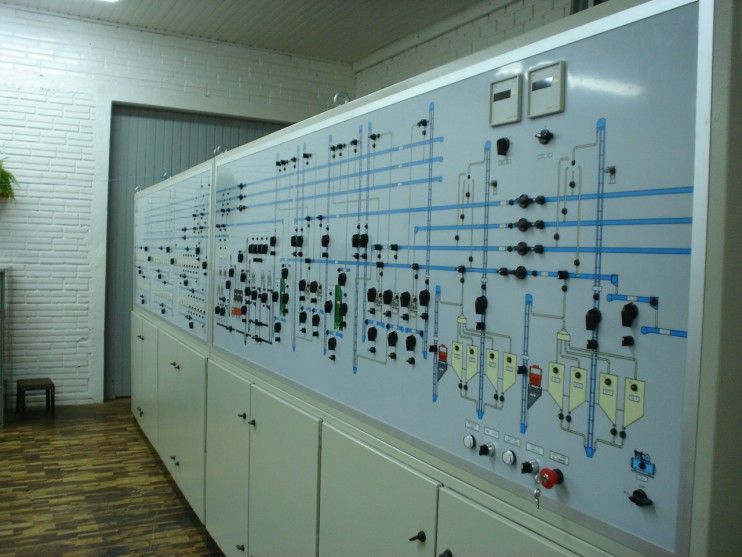
\includegraphics[width=0.6\textwidth]{figuras/painel_sinotico}
	\caption{Exemplo de um antigo painel sinótico.}\label{fig:painel_sinotico}
\end{figure}
Um sinótico é uma representação gráfica simplificada de um sistema -- uma síntese ótica. Num sistema SCADA, um sinótico representa uma área do processo em um certo nível de detalhe.

Tipicamente se tem um sinótico geral para uma planta, do qual se podem abrir sinóticos específicos de uma determinada área (numa hierarquia de sinóticos) ou a uma visão de uma outra camada do mesmo sinótico (por exemplo, um mostrando características elétricas e outro características termodinâmicas de um processo).

\begin{figure}[hb]
  \centering
  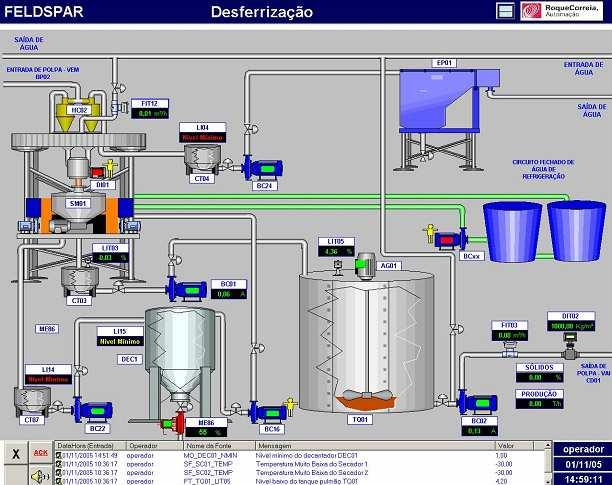
\includegraphics[width=0.6\textwidth]{figuras/sinotico_feldspar}
  \caption{Exemplo de um sinótico em um SCADA.}\label{fig:sinotico_feldspar}
\end{figure}


\subsection{Representação no sinótico}
\label{sub:Representação no sinótico}
Texto
Exibe valor de engenharia da variável analógica. A cor do texto pode servir
para codificar o status da variável.
• Barras horizontais e verticais
Fornecem uma representação percentual do valor da variável. Podem ser
utilizados para mostrar o enchimento de um silo, tanque, reator, etc.
• Deslocamento vertical, horizontal
Rotação
Efetua a rotação de um objeto: forno rotativo de cimento, pás de um
ventilador, etc associando 0° ao valor 0% da variáve l e 360° ao valor de
100%.
• Tendência
Exibe o gráfico dos últimos valores da variável em função do tempo.
• Mostradores Circulares

a) Texto
Exibe o status da variável: ABERTO/FECHADO ou LOCAL/REMOTO ou
LIGADO/DESLIGADO. Para cada estado é possível definir a cor de
apresentação do texto.
b) Associação a cor (ou outro atributo) de um objeto:
A cor do objeto muda de acordo com o status da variável associada.
c) Associação a um par de objetos complementares
Os dois objetos ocupam fisicamente a mesma posição no sinótico. Quando
a variável está em 0 o objeto chave aberta, por exemplo, é exibido, quando
está em 1 a chave é mostrada na posição fechada.

\subsection{Requisitos}
\label{sub:Requisitos}
Ao projetar uma IHM o projetista deve ter em mente:
a) Diminuir a chance de erro do operador principalmente nos
momentos de maior demanda operacional que coincide com o aumento
do stress:
b) Evitar as situações de monotonia que levam à desconcentração do
operador. Sinóticos pouco representativos do processo e sem atrações
de animação ou com muitos dados tabulares levem ao desinteresse.
c) Evitar situações que acarretam cansaço.
d) Manter o operador sempre atento ao que realmente interessa.
Evitar excesso de informações na tela. Sinóticos muito cheios trazem
excesso de informações que o operador não é capaz de processar. Os
alarmes e informações devem obedecer ao critério da exceção.
Avalanches de alarmes devem ser evitadas.
e) Evitar consulta a referências externas ao sistema. Se o operador
tiver dúvidas quanto a operação de elementos do sistema deverá
consultar o próprio sistema (Help on-line).

Conceitos ergonômicos para a construção de sinóticos :
• Os olhos tendem a se mover de:
Uma imagem grande para uma menor
Uma cor saturada para uma não saturada
Uma cor brilhante para um cor pastel
Uma imagem colorida para outra monocromática
Formas simétricas para formas assimétricas
Algo que se move e pisca para uma imagem estática.

A construção do sinóptico deve ser bem balanceada: o número de
elementos de informação por tela deve ser coerente com a capacidade
humana de interpretá-los. Evitar sinóticos congestionados ou vazios
demais.
• Representação gráfica dinâmica (animações).
• Evite objetos grandes piscantes
• Deve haver redundância na forma de representar uma informação:
valor, barras, enchimentos, etc. A representação mais natural é a mais
indicada. Por exemplo, enchimento para tanques e silos, rotação para um
forno de cimento ou britador de martelos, etc.

• Equipamentos devem ser desenhados de acordo com sua forma e
tamanhos exatos. A representação fotográfica com excesso de
detalhes, sombra, etc. é desaconselhável.
• A seqüência para ligar ou desligar equipamentos ou realizar ações
de controle similares deve ser simples e intuitiva. Simplesmente
selecione o objeto com o mouse e selecione a opção LIGA no menu.
IHMs de alguns terminais bancários são um bom contra exemplo.
• Mensagens devem ser claras, explícitas e auto suficientes. Contra
exemplo: Erro 46A: Execute o procedimento de emergência 78

\section{Alarmes e Eventos}
\label{sec:Alarmes e Eventos}


\section{Arquitetura de Hardware e Software}
\label{sec:Arquitetura de Hardware e Software}
